%% example text content
%% scrartcl and scrreprt starts with section, subsection, subsubsection, ...
%% scrbook starts with part (optional), chapter, section, ...
\chapter{Securing an Example Application}

In this chapter, the security concepts introduced above are put into practice by applying them to a real-world application. This application has been created solely for demonstration purposes to resemble a typical use case while still retaining simplicity to be generally applicable and easy to understand.

\section{Example Application}

\paragraph{Functionality}

The example application is a simple dashboard for Kubernetes to view Pods in certain or all namespaces. It can also display ReplicaSets and scale them up by demand. A screenshot of it is depicted in Figure \ref{fig:exaScreenshot}.

\begin{figure}[H]
\begin{center}
    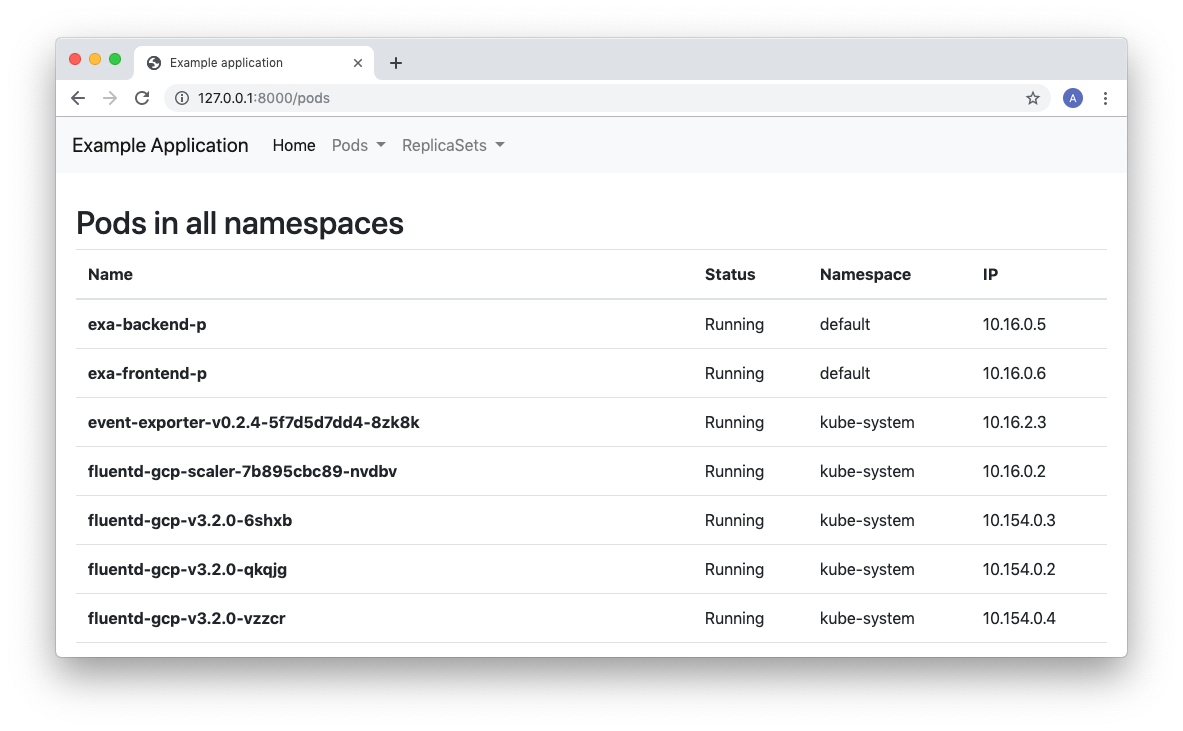
\includegraphics[width=1.0\linewidth]{figures/exa_screenshot.png}
    \caption[Screenshot of the example application]{This screenshot depicts the example application being port-forwarded to a local machine.}
    \label{fig:exaScreenshot}
\end{center}
\end{figure}

\paragraph{Setup}

The application is written in Python and makes use of Flask\footnote{\url{http://flask.pocoo.org/}, accessed 2019-07-02} as well as the Kubernetes Python Client\footnote{\url{https://github.com/kubernetes-client/python}, accessed 2019-07-02}. 

The setup consists of a backend \mycode{exa-backend} part and a frontend part \mycode{exa-frontend}. \mycode{exa-backend} provides a REST API with direct accesses to the Kubernetes API, while \mycode{exa-frontend} uses the backend for displaying the data. 

\begin{figure}[H]
\begin{center}
    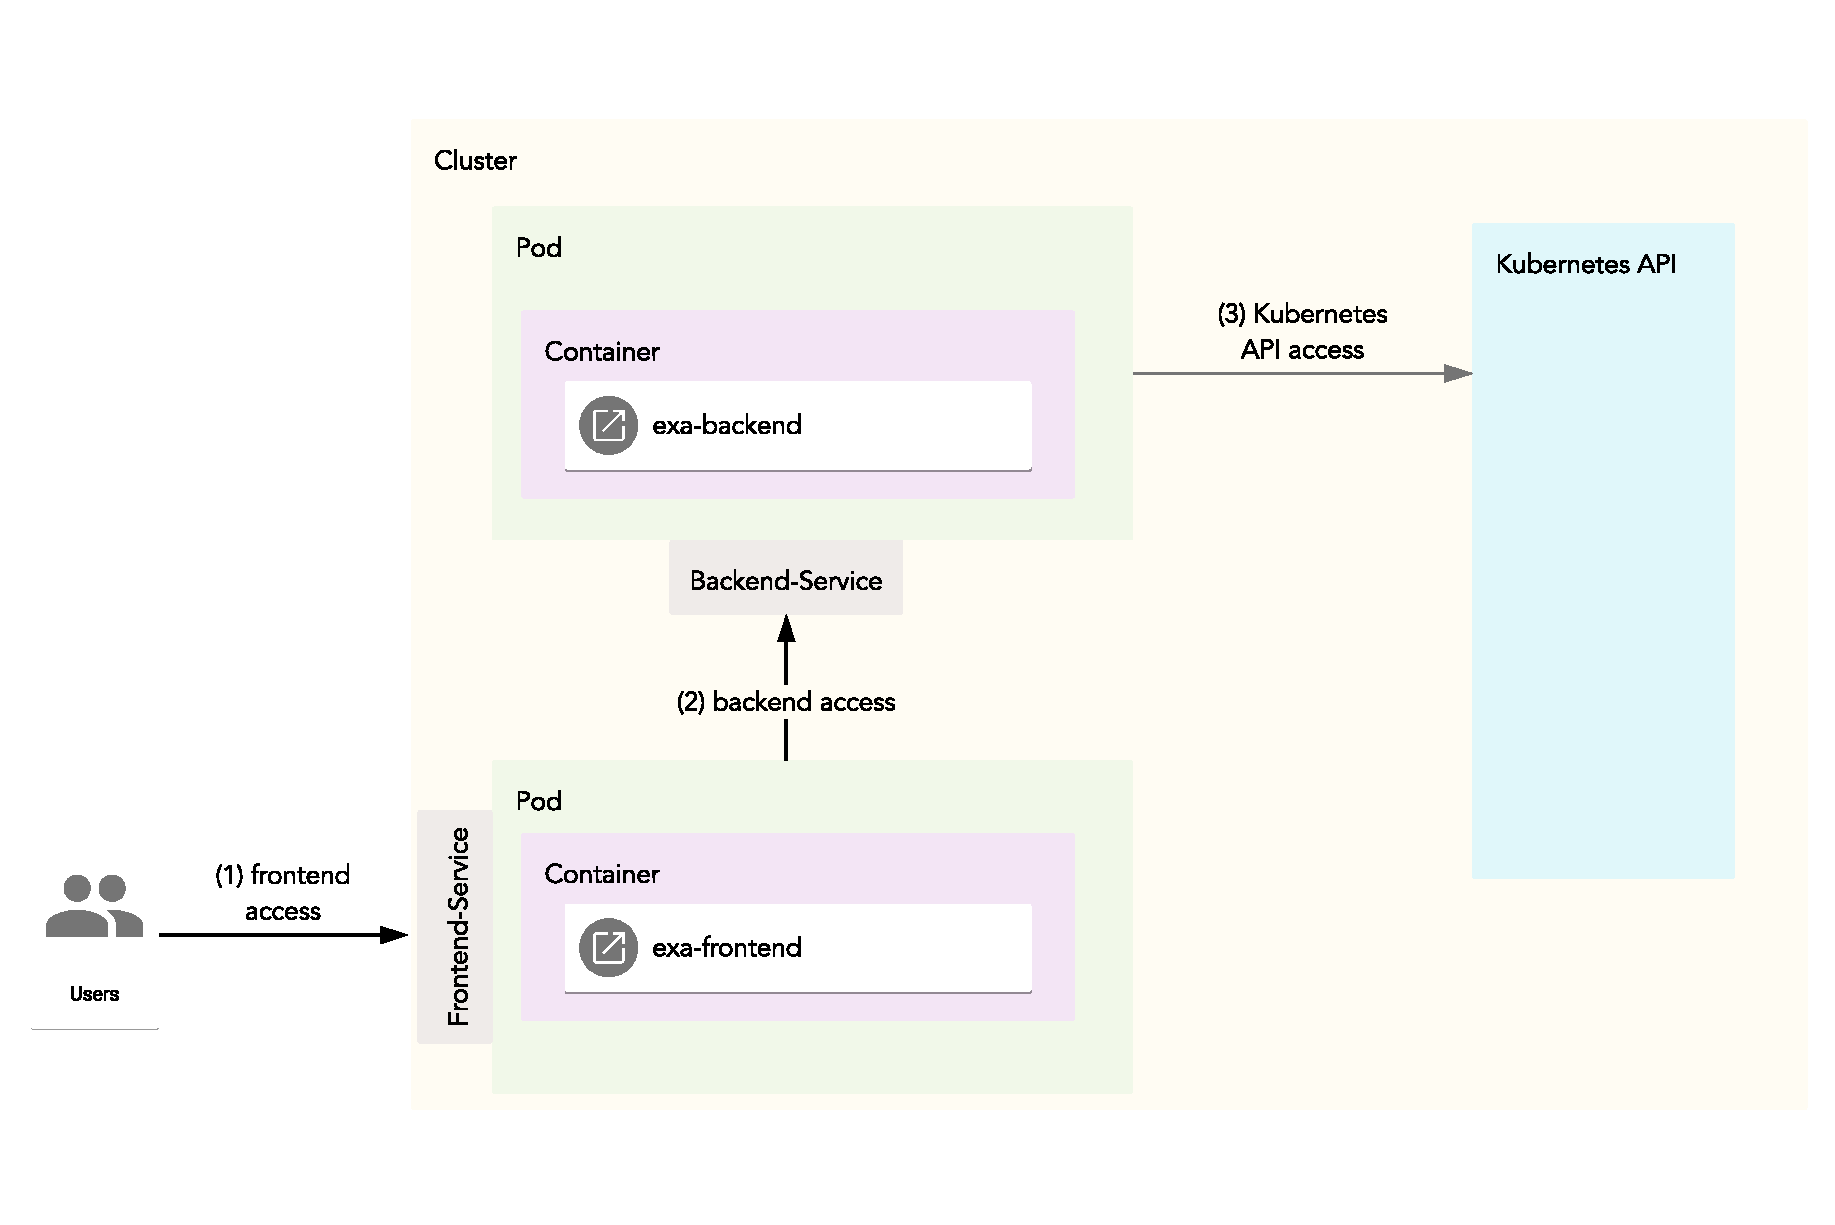
\includegraphics[width=1.0\linewidth]{figures/exa_architecture.pdf}
    \caption[Architecture of the example application]{This architecture diagram shows how the example application runs within the Kubernetes cluster.}
    \label{fig:exaArchitecture}
\end{center}
\end{figure}

The Kubernetes cluster is set up using \ac{GKE} on \ac{GCP}\footnote{\url{https://cloud.google.com/kubernetes-engine/}, accessed 2019-07-02}. It is a sensible choice for cluster administrators who are not yet experts in the field of Kubernetes security, as it scales well from a very basic setup up to a large high-availability cluster.

The architecture of the cluster is depicted in Figure~\ref{fig:exaArchitecture}. The frontend and backend components run in separate pods. Users access the frontend via an ingress that maps to the frontend service. The frontend then retrieves all information by calling the backend service, which in turn makes the request to the Kubernetes API to perform the user's query.

\section{Security Measures}

In this section, the measures that were taken to secure the setup are explained. They are structured according to the layer model introduced in Chapter~\ref{chap:clusterSecurity}.

\subsection{Base Infrastructure Security}

As this setup uses \ac{GKE} as an infrastructure provider, most considerations for base infrastructure security are already taken care of by Google\footnote{\url{https://cloud.google.com/kubernetes-engine/docs/concepts/security-overview}, accessed 2019-07-09}. By default, \ac{GKE} clusters run the newest version of Google's Container-Optimized OS\footnote{\url{https://cloud.google.com/container-optimized-os/docs/concepts/features-and-benefits}, accessed 2019-07-09} that comes with a current version of the container runtime as well. 

However, as all cluster components are running within the \ac{GCP} environment, they are also subject to Google's Cloud \ac{IAM}\footnote{\url{https://cloud.google.com/iam/}, accessed 2019-07-09}. It works alongside Kubernetes \ac{RBAC}, yet requires some special attention when applications within the Kubernetes cluster access other resources on \ac{GCP} outside of the cluster.\footnote{\url{https://cloud.google.com/kubernetes-engine/docs/how-to/iam}, accessed 2019-07-09}

\subsection{Kubernetes Infrastructure Security}

\paragraph{API Server}

When it comes to the security of Kubernetes infrastructure, namely the API server, the aforementioned \ac{IAM} can also cause potential weaknesses, if not correctly configured. When it is used as the means for authorisation, by default, log in using username and password is allowed. We disabled it in the cluster configuration in the \ac{GCP} web interface and only used certificates, which we regularly rotate\footnote{\url{https://cloud.google.com/kubernetes-engine/docs/how-to/credential-rotation}, accessed 2019-07-09}, to authenticate within the cluster.

\paragraph{Secret Encryption}

As explained in Section~\ref{ssec:etcd}, it is vital to encrypt all secrets stored in \mycode{etcd}. While \ac{GKE} uses encryption at rest by default\footnote{\url{https://cloud.google.com/security/encryption-at-rest/default-encryption/}, accessed 2019-07-09}, we also configured application-layer encryption in case an attacker gains access to an offline copy of the \mycode{etcd} database. To set up the encryption, we generated a key, stored it in Google's Cloud Key Management Service (KMS)\footnote{\url{https://cloud.google.com/kms/docs/}, accessed 2019-07-09} and handed it to the cluster configuration using \mycode{--database-encryption-key}\footnote{\url{https://cloud.google.com/kubernetes-engine/docs/how-to/encrypting-secrets}, accessed 2019-07-09}.  

\paragraph{Dashboard}

As the standard Kubernetes dashboard is deprecated and disabled by default on GKE, no further configuration was necessary to secure the setup. The \ac{GCP} Console\footnote{\url{https://console.cloud.google.com/}, accessed 2019-07-09}, which acts as a replacement for the standard dashboard on \ac{GKE}, again uses Google's \ac{IAM} and therefore needs no further protection. It is conceptually not accessible by unauthenticated users. 

\subsection{Kubernetes Security Controls}
% TODO write

\subsection{App and Container Security}
% TODO write

%% vim:foldmethod=expr
%% vim:fde=getline(v\:lnum)=~'^%%%%\ .\\+'?'>1'\:'='
%%% Local Variables: 
%%% mode: latex
%%% mode: auto-fill
%%% mode: flyspell
%%% eval: (ispell-change-dictionary "en_US")
%%% TeX-master: "main"
%%% End: 
